\documentclass[a4paper]{article}
\usepackage[a4paper,margin=0mm]{geometry}
\usepackage{fontspec}
\usepackage{unicode-math}
\usepackage{tikz}
\usetikzlibrary{fit,calc,positioning,arrows.meta}
\usepackage[table]{xcolor}
\usepackage[absolute]{textpos}
\usepackage{array}

\setmainfont{Libertinus Serif}
\setsansfont{Libertinus Sans}
\setmathfont{Libertinus Math}

\definecolor{accent}{HTML}{602785}
\definecolor{badge}{HTML}{B8A0C8}
\definecolor{ink}{HTML}{2A2E30}

\setlength{\TPHorizModule}{1mm}
\setlength{\TPVertModule}{1mm}
\setlength{\parindent}{0pt}
\pagestyle{empty}

\newcommand{\topicheader}[2]{%
\begin{textblock*}{194mm}(16mm,10mm)
\begin{tikzpicture}
\node[fill=accent,text=white,font=\sffamily\bfseries\fontsize{13}{13}\selectfont,
      minimum width=9mm,minimum height=9mm,inner sep=0pt] at (4.5mm,-4.5mm) {#1};
\node[font=\sffamily\bfseries\fontsize{15}{16}\selectfont,text=ink,anchor=west] at (12mm,-4.5mm) {#2};
\end{tikzpicture}
\end{textblock*}
\begin{textblock*}{194mm}(16mm,22.5mm)

\begin{tikzpicture}
\fill[accent] (0,0) rectangle (194mm,0.5mm);
\end{tikzpicture}
\end{textblock*}
}

\newcommand{\pagekicker}[1]{%
\begin{textblock*}{100mm}(16mm,25.5mm)
\begin{tikzpicture}
\node[fill=ink,text=white,font=\sffamily\bfseries\fontsize{8}{8}\selectfont,
      inner sep=2.2pt,rounded corners=1pt] {\MakeUppercase{#1}};
\end{tikzpicture}
\end{textblock*}
}

\newcommand{\videobanner}[1]{%
\begin{textblock*}{178mm}(16mm,25.5mm)
\begin{tikzpicture}
\fill[accent] (0,0) rectangle (178mm,-10mm);
\draw[white,line width=0.6pt] (3mm,-1.7mm) rectangle (11.5mm,-8.3mm);
\node[white,font=\sffamily\fontsize{4}{4.4}\selectfont,align=center] at (7.25mm,-5mm) {QR\\CODE};
\node[white,font=\sffamily\bfseries\fontsize{9.5}{11}\selectfont,anchor=west] at (16mm,-5.6mm) {WATCH THE VIDEO BEFORE YOU SOLVE};
\node[white,font=\sffamily\fontsize{7.5}{8}\selectfont,anchor=east] at (174mm,-5.6mm) {YouTube ~\textbullet~ #1};
\end{tikzpicture}
\end{textblock*}
}

\newcommand{\pagefooter}[1]{%
\begin{textblock*}{194mm}(8mm,286.41mm)
  
\begin{tikzpicture}
    \fill[accent] (0,0) rectangle (194mm,0.6mm);
  \end{tikzpicture}
\end{textblock*}
\begin{textblock*}{63.59mm}(8mm,288.27mm)
  {\sffamily\bfseries\color{accent}\fontsize{13}{16}\selectfont SAT 1200+}
\end{textblock*}
\begin{textblock*}{10mm}(188mm,288.27mm)
  \centering{\sffamily\color{accent}\fontsize{14}{16}\selectfont #1}
\end{textblock*}
}

\newcommand{\cardbg}[4]{%
\begin{textblock*}{#3mm}(#1mm,#2mm)
\begin{tikzpicture}
\fill[badge!22,rounded corners=3mm] (0,0) rectangle (#3mm,-#4mm);
\end{tikzpicture}
\end{textblock*}%
}

\newcommand{\pill}[3]{%
\begin{textblock*}{160mm}(#1mm,#2mm)
\begin{tikzpicture}
\node[fill=accent,text=white,anchor=north west,font=\sffamily\bfseries\fontsize{10}{10}\selectfont,
      rounded corners=8pt,inner xsep=5mm,inner ysep=1.8mm] at (0,0) {RULE ~\textperiodcentered~ #3};
\end{tikzpicture}
\end{textblock*}%
}

\arrayrulecolor{accent}
\setlength{\arrayrulewidth}{0.7pt}
\renewcommand{\arraystretch}{1.5}

\begin{document}

% ======================================================================
% PAGE 1
% ======================================================================
\topicheader{19}{Angles \& Triangles}
\videobanner{Lesson 19}
\pagefooter{103}
\mbox{}%

% ---- CARD 1: Angle relationships ----
\cardbg{16}{40}{178}{70}
\pill{26}{43}{Angle relationships (burchaklar)}

\begin{textblock*}{158mm}(26mm,56mm)
{\fontsize{11}{14}\selectfont
\begin{tabular}{|p{60mm}|>{\centering\arraybackslash}p{85mm}|}
\hline
\rowcolor{accent}
{\color{white}\textbf{Type}} & {\color{white}\textbf{Rule}} \\ \hline
Complementary & sum $=90°$ \\ \hline
Supplementary & sum $=180°$ \\ \hline
Vertical angles & equal \\ \hline
\end{tabular}}
\end{textblock*}

\begin{textblock*}{158mm}(26mm,95mm)
{\fontsize{13}{16}\selectfont $\angle A+\angle B+\angle C=180°$ (any triangle)}
\end{textblock*}

% ---- CARD 2: Parallel lines cut by a transversal ----
\cardbg{16}{116}{178}{150}
\pill{26}{119}{Parallel lines cut by a transversal}

\begin{textblock*}{158mm}(26mm,132mm)
{\fontsize{11}{14}\selectfont
\begin{tabular}{|p{60mm}|>{\centering\arraybackslash}p{85mm}|}
\hline
\rowcolor{accent}
{\color{white}\textbf{Pair}} & {\color{white}\textbf{Rule}} \\ \hline
Corresponding angles & equal \\ \hline
Alternate interior angles & equal \\ \hline
Co-interior (same-side) angles & sum $=180°$ \\ \hline
\end{tabular}}
\end{textblock*}

\begin{textblock*}{158mm}(26mm,171mm)
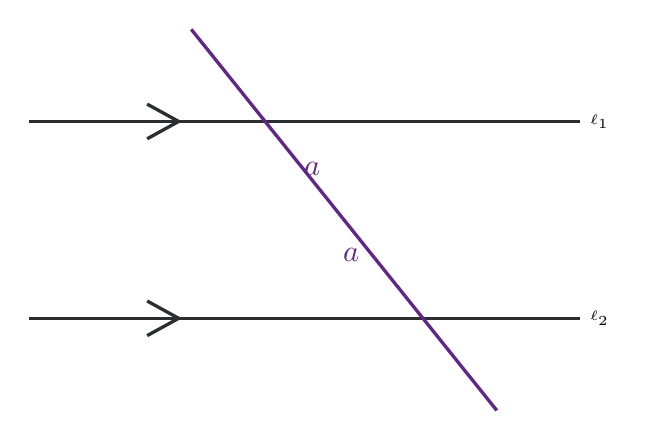
\begin{tikzpicture}[every node/.style={font=\fontsize{10}{10}\selectfont}]
\coordinate (L1a) at (-5mm,25mm); \coordinate (L1b) at (65mm,25mm);
\coordinate (L2a) at (-5mm,0mm);  \coordinate (L2b) at (65mm,0mm);
\draw[ink,line width=1pt] (L1a) -- (L1b);
\draw[ink,line width=1pt] (L2a) -- (L2b);
\draw[ink,line width=1.2pt] (10mm,22.8mm) -- (14mm,25mm) -- (10mm,27.2mm);
\draw[ink,line width=1.2pt] (10mm,-2.2mm) -- (14mm,0mm) -- (10mm,2.2mm);
\coordinate (P) at (25mm,25mm); \coordinate (Q) at (45mm,0mm);
\draw[accent,line width=1.2pt] (15.6mm,36.7mm) -- (54.4mm,-11.7mm);
\node[text=accent,font=\sffamily\bfseries\fontsize{11}{11}\selectfont] at (31mm,19mm) {$a$};
\node[text=accent,font=\sffamily\bfseries\fontsize{11}{11}\selectfont] at (36mm,8mm) {$a$};
\node[anchor=west,font=\tiny] at (65mm,25mm) {$\ell_1$};
\node[anchor=west,font=\tiny] at (65mm,0mm) {$\ell_2$};
\end{tikzpicture}
\end{textblock*}

\begin{textblock*}{158mm}(26mm,245mm)
{\fontsize{10}{13}\selectfont\color{black!55}\itshape
Only applies when the lines are stated or marked ($\rightarrow$) parallel -- never assume
from how a figure looks.}
\end{textblock*}

\clearpage

% ======================================================================
% PAGE 2
% ======================================================================
\topicheader{19}{Angles \& Triangles}
\pagekicker{Rules sheet -- 2/2}
\pagefooter{104}
\mbox{}%

% ---- CARD 3: Similar triangles ----
\cardbg{16}{33}{178}{80}
\pill{26}{36}{Similar triangles (o'xshash)}

\begin{textblock*}{158mm}(26mm,49mm)
{\fontsize{12}{15}\selectfont
$\triangle ABC\sim\triangle DEF\ \Longrightarrow\ \dfrac{AB}{DE}=\dfrac{BC}{EF}=\dfrac{AC}{DF}$}
\end{textblock*}

\begin{textblock*}{158mm}(26mm,68mm)
{\fontsize{11}{14}\selectfont\color{ink}
Letter order tells you the match: $A\leftrightarrow D$, $B\leftrightarrow E$, $C\leftrightarrow F$
-- proportional, not equal.}
\end{textblock*}

\begin{textblock*}{158mm}(26mm,80mm)
{\fontsize{11}{14}\selectfont
$AB=6,BC=9,AC=12,DE=8\ \Longrightarrow\ \text{scale}=\dfrac{8}{6}=\dfrac43\ \Longrightarrow\ EF=12,\ DF=16$}
\end{textblock*}

% ---- CARD 4: Proving similarity ----
\cardbg{16}{122}{178}{110}
\pill{26}{125}{Proving similarity}

\begin{textblock*}{158mm}(26mm,138mm)
{\fontsize{11}{14}\selectfont
\begin{tabular}{|>{\centering\arraybackslash}p{20mm}|p{125mm}|}
\hline
\rowcolor{accent}
{\color{white}\textbf{Test}} & {\color{white}\textbf{Checks}} \\ \hline
AA & two pairs of angles equal \\ \hline
SAS & two side pairs proportional, included angle equal \\ \hline
SSS & all three side pairs proportional \\ \hline
\end{tabular}}
\end{textblock*}

\begin{textblock*}{158mm}(26mm,180mm)
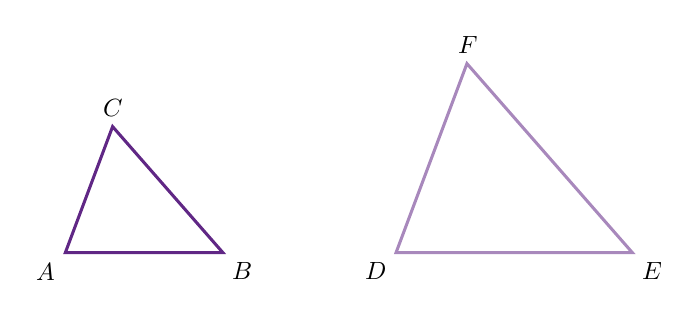
\begin{tikzpicture}[every node/.style={font=\fontsize{9}{9}\selectfont}]
\coordinate (A) at (0mm,0mm); \coordinate (B) at (20mm,0mm); \coordinate (C) at (6mm,16mm);
\coordinate (D) at (42mm,0mm); \coordinate (E) at (72mm,0mm); \coordinate (F) at (51mm,24mm);
\draw[accent,line width=1.1pt] (A) -- (B) -- (C) -- cycle;
\draw[accent!55,line width=1.1pt] (D) -- (E) -- (F) -- cycle;
\node[anchor=north east] at (A) {$A$};
\node[anchor=north west] at (B) {$B$};
\node[anchor=south] at (C) {$C$};
\node[anchor=north east] at (D) {$D$};
\node[anchor=north west] at (E) {$E$};
\node[anchor=south] at (F) {$F$};
\end{tikzpicture}
\end{textblock*}

\begin{textblock*}{158mm}(26mm,218mm)
{\fontsize{10}{13}\selectfont\color{black!55}\itshape
Same shape, different size -- angles match exactly, sides scale by one constant factor.}
\end{textblock*}

\end{document}
